\subsection*{Problem 13-4 Treaps}
\begin{enumerate}
	\item	对于一棵BST,可以对每个节点进行Rotation,所有这些BST与原始的BST都是同构的,然而在Treap中,这棵树要满足Heap的性质,所以不能进行Rotation,即这棵BST是确定唯一的
	\item	对于所有节点的priority序列,每一种排列都唯一的对应一种Treap,即所有节点以一种排列顺序插入所形成的BST,因为所有的节点的priority都是随机产生的,所以Treap的本质就是Randomly built binary search trees,所以the expected height of a treap is $\Theta(\log{n})$
	\item	the procedure $\proc{Treap-Insert}$ consist of $\proc{BST-Tree-Insert}$ and $\proc{Heap-Increase-Key}$ by $\proc{Rotation}$
	\item	$\proc{BST-Tree-Insert}$: $\mathcal{O}(\log{n})$ \\
		$\proc{Heap-Increase-Key}$: $\mathcal{O}(\log{n})$ ($\proc{Rotation}$: $\mathcal{O}(1)$) \\
		$\proc{Treap-Insert}$ Total: $\mathcal{O}(\log{n})$
	\item	对于一个leaf node $x$,可以归纳,每次对于$x$进行一次Rotation,其$C + D$会增加1,归纳过程如图 \\
		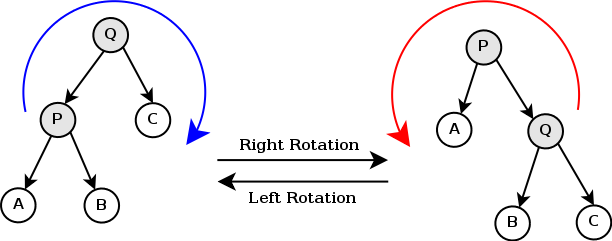
\includegraphics[width=10cm]{chapter13/Tree_rotation.png} \\
		对于Right-Rotation,设节点$x$为$P$,$A, B$分别为$x$的左右两棵子树,$Q$是$P$的parent,$C$是$Q$的右子树,原始的$C + D = left\_spine(B) + right\_spine(A)$,经过Right-Rotation后,$C' + D' = right\_spine(A) + 1 + left\_spine(B)$ \\
		同理,Left-Rotation亦是如此,即对于插入树中的节点$x$,其Rotation的次数等于$C + D$
	\item	(Omit!)
	\item	\begin{equation} \notag
			Pr\{X_{ik} = 1\} = \frac{(k - i - 1)!}{(k - i + 1)!} = \frac{1}{(k - i + 1)(k - i)}
		\end{equation}
	\item	\begin{equation} \notag
			E[C] = \sum_{i = 1}^{k - 1} Pr\{X_{ik} = 1\} = \sum_{i = 1}^{k - 1} \frac{1}{(k - i + 1)(k - i)} = \sum_{j = 1}^{k - 1} \frac{1}{j(j + 1)} = 1 - \frac{1}{k}
		\end{equation}
	\item	由对称性,令$k = n - k + 1$即可,即
		\begin{equation} \notag
			E[D] = 1 - \frac{1}{n - k + 1}
		\end{equation}
	\item	因为$E[C + D] = E[C] + E[D] < 2$,所以当向Treap中插入一个节点时,期望的Rotation次数小于2
\end{enumerate}

